\documentclass{uflamon}          % classe base para a monografia

%==============================================================================
% Utilizacao de pacotes
\usepackage[T1]{fontenc}         % usa fontes postscript com acentos
\usepackage[brazil]{babel}       % hifenização e títulos em português do Brasil
\usepackage[utf8]{inputenc}     % permite edição direta com acentos
\usepackage{amsmath}             % pacote da AMS para Matemática Avançada
\usepackage{amssymb}             % símbolos extras da AMS
\usepackage{latexsym}            % símbolos extras do LaTeX
\usepackage{graphicx}            % para inserção de gráficos
\usepackage{listings}            % para inserção de código
\usepackage{fancyvrb}            % para inserção de saídas de comandos
%\usepackage{enumerate}           % para personalizar lista enumeradas 
											%(incluso na classe)
\usepackage{longtable}           % para tambelas muito grandes NOVO!!!!

\usepackage{colortbl} % cores em tabelas
\newcolumntype{Z}{|>{\columncolor[gray]{0.9}}l|} %cor cinza em células
%\usepackage{array} % já incluso na classe
\newcolumntype{L}[1]{>{\raggedright\let\newline\\\arraybackslash\hspace{0pt}}m{#1}}
\newcolumntype{C}[1]{>{\centering\let\newline\\\arraybackslash\hspace{0pt}}m{#1}}
\newcolumntype{R}[1]{>{\raggedleft\let\newline\\\arraybackslash\hspace{0pt}}m{#1}}
\usepackage{multirow} % para juntar duas linhas em uma só

\usepackage{multicol} % para uso de várias colunas

% cores para os links cruzados
\usepackage{color}
\definecolor{rltred}{rgb}{0.2,0,0}
\definecolor{rltgreen}{rgb}{0,0.2,0}
\definecolor{rltblue}{rgb}{0,0,0.2}

\usepackage[colorlinks=true,
            urlcolor=rltblue,       % \href{...}{...} external (URL)
            filecolor=rltgreen,     % \href{...} local file
            linkcolor=rltred,       % \ref{...} and \pageref{...}
            citecolor=rltgreen,
            pdftitle={Exemplo de Uso da Classe Uflamon},
          pdfauthor={Joaquim Quinteiro Uchôa},
          pdfsubject={Este texto tem por objetivo servir de exemplo da classe Uflamon.},
          pdfkeywords={Comunicação Científica. 2. Pesquisa . 3. Pesquisa Científica. 
 					 4. Redação. 5. Monografia.}%
]{hyperref} % para referência cruzadas
%\usepackage{hyperref}            % para referência cruzadas
\usepackage{subfigure}           % figuras dentro de figuras
\usepackage{caption}            % remodelando o formato dos títulos de 
                                 % tabelas e figuras

% configuração padrão do listings   
\lstset{
   language=Java,
   extendedchars=true,
   tabsize=3,
   basicstyle=\footnotesize\ttfamily,
   stringstyle=\em,
   showstringspaces=false 
}

% para referências de acordo com a ABNT
% precisa instalar o abntex2 antes!!!
% http://abntex.codigolivre.org.br/
% comente se pretende usar outro padrão

%abnt-emphasize=bf coloca o título das bibliografias em negrito
%abnt-thesis-year=both
\usepackage[alf,abnt-etal-cite=3,abnt-etal-list=3,abnt-url-package=url,abnt-emphasize=bf]{abntex2cite}

% evite usar o hyperref com abntex, pode dar caca em urls... no linha anterior, informo
% para incluir urls usando o pacote url e não o hyperref
%
% caso queira o hyperref com abntex, comente a linha anterior e descomente a seguinte
%\usepackage[alf,abnt-etal-cite=3,abnt-etal-list=0,abnt-etal-text=emph]{abntex2cite}
%
% caso vc ainda use a versão anterior da abntex, comente a linha incluindo o abntex2cite
% e descomente a próxima linha 
%\usepackage[alf,abnt-etal-cite=3,abnt-etal-list=0,abnt-etal-text=emph]{abntcite}


% redefinindo formatação de títulos de tabelas e figuras


%==============================================================================
% para os fãs do Word, descomente as linhas abaixo
%\sloppy %mais espaço entre as linhas
%\usepackage{identfirst} %identando-se a primeira linha de cada seção
%\noindentfirst % Tire o comentário para manter o padrão do LaTeX.

%==============================================================================
% definido comandos na monografia - não é necessário na sua monografia 
% apenas para exemplificar a definição de novos comandos
\newcommand{\defs}[1]{\textsl{#1}}


% Especificando hifenizações que por ventura LaTeX não saiba fazer
% Por padrão 99,9% dos termos em português devem ser hifenizados corretamente.
\hyphenation{hardware software Li-nux am-bien-te diag-nos-ti-car coor-de-na-ção 
FAE-PE Recovery TelEduc Williams UFLA}

%==============================================================================
% Dados da monografia, capa: autor, titulo, banca, etc... - SUBSTITUA DE ACORDO
%==============================================================================
\author{Joaquim Quinteiro Uchôa}
\title{Uso da Classe Uflamon}
\subtitle{Exemplo para os Usuários}
\engtitle{Use of Uflamon Class}
\engsubtitle{Sample for Users}
\edicao{3$^a$ edição revista, atualizada e ampliada}
\date{2016}
\tipo{Tese apresentada à Universidade Federal de Lavras, como parte das exigências do Programa de Pós-Graduação em Monografia, área de concentração em TCC, para a obtenção do título de Doutor.}
% use \orientador ou \orientadora quando for o caso
\orientador{Prof. DSc. José Orientador}
%\orientadora{}
% use \coorientador ou \coorientadora quando for o caso
%\coorientadora{Prof. DSc. Maria Orientadora } % comente se não tiver coorientador
%\coorientador{}
\local{Lavras -- MG}
%\bancaum{Prof. MSc. Antônio Banca Um}{UFM}
%\bancadois{Prof. DSc. João Banca Dois}{FCO} % comente se sua banca tiver só um professor
%\bancatres{Profa. Esp. Eliza Banca Três}{BELMIS}
%\bancaquatro{Prof. Esp. Carlos Banca Quatro}{IBGPLUS}
%\defesa{30 de Fevereiro de 2016}
%==============================================================================
%##################################################
% Dados para Ficha catalográfica, gerada pelo sistema da Biblioteca da UFLA
% http://www.biblioteca.ufla.br/FichaCatalografica/
% dados para ficha catalográfica
% Elaboração da Ficha Catalográfica
%\preparofichacat{Ficha catalográfica elaborada pela Coordenadoria de Processos Técnicos \\ da Biblioteca Universitária da UFLA}
% primeiro autor - como na primeira linha da ficha catalográfica
%\fcautor{Uchôa, Joaquim Quinteiro}
% autores, separados por vírgula - na ficha catalográfica, no formato que
% vem após o título e a barra ("/")
%\fcautores{Joaquim Quinteiro Uchôa}
% caso trabalho seja ilustrado (figuras, gráficos, tabelas, etc.), 
% então informar por meio do comando a seguir
% caso não seja ilustrado, basta comentá-lo
%\fcilustrado{il.}
% dados da edição para a ficha 
%\fcedicao{2$^a$ ed. rev., atual. e ampl.}
% tipo do trabalho (tese, dissertação, etc.), de acordo com sistema
% de geração de ficha catalográfica
%\fctipo{Tese(doutorado)}
% ano da defesa, só precisa informar se for diferente do ano da publicação
% se forem iguais, comente a linha a seguir
%\fcdatadefesa{2016}
% preencher aqui com os dados de catalogação gerados pelo sistema
%\fccatalogacao{1. TCC. 2. Monografia. 3. Dissertação. 4. Tese. 5. Trabalho Científico – Normas. I. Universidade Federal de Lavras. II. Título.}
%\fcclasi{808.066}

%##################################################

%\antesfichacat{\noindent Para citar este documento: \\UNIVERSIDADE FEDERAL DE LAVRAS. Biblioteca Universitária. \textbf{Manual de normalização e estrutura de trabalhos acadêmicos: TCC, monografias, dissertações e teses}. 2. ed. rev., atual. e ampl. Lavras, 2015. Disponível em: \url{http://www.biblioteca.ufla.br/wordpress/wpcontent/uploads/bdtd/manual_normalizacao_UFLA.pdf}. Acesso em: data de acesso.}

%\depoisfichacat{\noindent A reprodução e a divulgação total ou parcial deste trabalho são autorizadas, por qualquer meio convencional ou eletrônico, para fins de estudo e pesquisa, desde que citada a fonte.\\
%\newline
%{\small Este documento possui páginas em branco para facilitar a impressão frente-e-verso.}}

%##################################################

%##################################################

% para os exemplos do manual
%\newenvironment{exemplomanual}{
%\vspace{0.5cm}
%\noindent\begin{minipage}{\textwidth}
%\noindent\rule{\textwidth}{0.5pt}
%\vspace{-1cm}
%\begin{flushleft}
%}{
%\end{flushleft}
%\vspace{-0.6cm}
%\noindent\rule{\textwidth}{0.5pt}
%\vspace{0.3cm}
%\end{minipage}
%}

%\newenvironment{exemplomanuallista}{
%\vspace{0.3cm}
%\noindent\begin{minipage}{\textwidth - 0.5cm}
%\noindent\rule{\textwidth}{0.5pt}
%\vspace{-1cm}
%\begin{flushleft}
%}{
%\end{flushleft}
%\vspace{-0.6cm}
%\noindent\rule{\textwidth}{0.5pt}
%\vspace{0.3cm}
%\end{minipage}
%}

% por conta de alguns exemplos
%\usepackage{setspace}

%##################################################

% se vc já defendeu e tem o arquivo escaneado da folha de rosto, 
% descomente e altere o nome do arquivo
%\folhaAprovacaoAssinada{folharosto}

% Aqui começa o documento propriamente dito
\begin{document}

\maketitle

\dedic{Espaço reservado a dedicatória.}     % Dedicatórias\\

\thanks{Espaço reservado aos agradecimentos.}         % Agradecimentos

\epigrafe{ % citação opcional
Espaço reservado a epígrafe.\\
(Autor Desconhecido)}

% palavras-chave
\palchaves{Resumo. Palavras. Representativas.}
\resumo{O resumo deve conter palavras representativas do conteúdo do trabalho, localizadas abaixo do resumo, separadas por dois espaços, antecedidas da expressão palavras-chave. Essas palavras representativas são grafadas com a letra inicial em maiúscula, separadas entre si por ponto.}  % Resumo (digite aqui o resumo)

% keywords devem vir antes do abstract
\keywords{Summary. Words. Representative.} % keywords
\abstract{The abstract should contain representative words of the work content, located below the abstract, separated by two spaces, preceded by the keyword expression. These representative words are spelled with the first letter capitalized, separated by point.}

%##################################################

% Dados do guia
%\begin{titlepage}
%\pagestyle{empty}
%\renewcommand{\baselinestretch}{1}
%\enlargethispage{1.5cm}
%\input{reitoria}
%\cleardoublepage
%\end{titlepage}

%##################################################

% descomente para habilitar a lista desejada
\listoffigures                             % Lista de Figuras
%\listofilustracoes
%\listofgraficos							   % Lista de Gráficos
\listoftables                              % Lista de Tabelas
\listofquadros							   % Lista de Quadros
%\listofexemplos
%\listofteoremas
\tableofcontents                           % Sumário

\clearpage

\pagestyle{ufla}

%==============================================================================
% incluindo os capitulos
\chapter{Introdução}\label{intro}
\section{Justificativa}\label{sub:just}    

O ácido acetilsalicílico é, possivelmente, o medicamento mais conhecido e vendido no mundo todo.
Desse modo, a análise dos comprimidos comercializados é de interesse dos estudantes da Engenharia
Química, uma vez que proporciona aprendizado a cerca da indústria farmacêutica, padrões de
qualidade, além de práticas laboratoriais da teoria de química analítica e orgânica.

\section{Objetivos}\label{sub:Objetivos}
Determinar o teor de ácido acetilsalicílico contido nos comprimidos comercializados, analisando
medicamentos de referência (Aspirina\R), genéricos e similares.

\section{Referencial Teórico}\label{sub:reft}

\subsection{Histórico}\label{sub:Histórico}

O ácido acetilsalicílico (AAS) é um dos medicamentos mais populares no mundo, sendo conhecido por
seu nome comercial: Aspirina\R. Ele é um analgésico, anti-inflamatório e antipirético produto de uma
reação que tem como um dos reagentes o ácido salicílico, extraído do salgueiro (\textit{Salix
alba}).  

O ácido acetilsalicílico pode ser identificado também pela sua fórmula química \ce{C9H8O4} e seu
nome IUPAC ácido 2-acetóxibenzóico. É um ácido de caráter fraco por apresentar-se,
predominantemente, em sua forma não ionizada. Demonstra características de um ácido orgânico e de
éster, pois ambas as estruturas existem em sua fórmula molecular. A respeito de propriedades
físico-químicas, o AAS é um pó cristalino branco, inodoro, solúvel em álcool e éter e pouco solúvel
em água devido à massa molar elevada de 180,157g/mol, sendo a relação de sua solubilidade em água
0,3g/100g (25$^\circ$C). Ele possui ponto de fusão 135$^\circ$C e ponto de ebulição a 140$^\circ$C.
Ecologicamente, é facilmente biodegradado em estações de tratamento de água e não
bioacumula.~\cite{teves}

\begin{figure}[H]
\begin{center}
    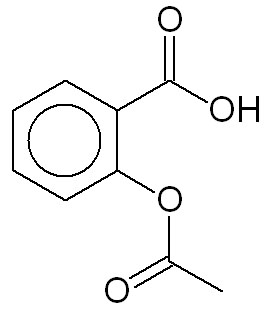
\includegraphics[scale=.4]{figuras/acido_acetilsalicilico.jpg}
\end{center}
\caption{Ácido acetisalicílico}
\label{fig:acid_AAS}
\end{figure}


A utilização do ácido salicílico, no alívio de dores já existe há séculos, isso porque essa
substância está contida em diversas plantas consideradas medicinais. “Uma coleção de anotações
datadas de cerca de 1500 a.C., conhecidas como papiros de Ebers, já recomendava o uso da infusão de
folhas de murta para o alívio de dores reumáticas”~\cite{aspirinabayer}. Posteriormente, no século V
a.C., Hipócrates, o pai da medicina moderna, registrou que o pó da casca do salgueiro era capaz de
amenizar dores e febre. Somente em 1860 a substância encontrada na casca do salgueiro foi isolada em
laboratório e recebeu o nome de salicilato, que designa um “grupo de fármacos que atuam devido ao
seu conteúdo de ácido salicílico”.~\cite{Goodman2005}

Já o descobrimento do ácido acetilsalicílico ocorreu mais tarde, “quando o químico alemão Felix
Hoffman pesquisava um medicamento para ser usado no tratamento da artrite, doença de seu pai. O
objetivo dele era encontrar uma droga para substituir o salicilato de sódio, medicamento usado
naquela época, mas que exigia grandes doses diárias e provocava irritação e fortes dores estomacais
nos pacientes”.~\cite{massabni2006}

Em 1897, Hoffman, que trabalhava na companhia Bayer da Alemanha, preparou o ácido acetilsalicílico
combinando o ácido salicílico com acetato. A reação resultou numa substância mais vantajosa do que o
salicilato de sódio, em questão de eficiência e efeitos colaterais. Tal droga recebeu,
posteriormente, o nome de Aspirina\R e se tornou o primeiro fármaco sintetizado em laboratório.  

A Aspirina\R teve sua patente concedida em 1899 e começou a ser comercializada.  Ainda que
inicialmente os superiores de Hoffman achassem que o medicamento fracassaria, o mesmo tornou-se
sucesso de vendas e inclusive destacou-se como medicamento mais utilizado no tratamento da artrite.
Inicialmente, a Aspirina\R era vendida na forma de pó, entretanto, em 1900, ela tornou-se o primeiro
medicamento no mundo a ser vendido em doses padronizadas, que eram comprimidos com 500mg de ácido
acetilsalicílico. “A formulação em comprimidos tinha três vantagens principais: assegurar que cada
comprimido tivesse uma dose exata do ingrediente ativo, acabar com as falsificações dos produtos e
reduzir os custos de produção".~\cite{aspirinabayer}

Décadas depois, John Vane, Professor de Farmacologia do London Royal College for Surgeons, “observou
que alguns tipos de ferimento eram acompanhados da liberação em nosso corpo de substâncias chamadas
de prostaglandinas. Ele também percebeu que dois grupos delas provocavam febre e vermelhidão no
local do ferimento (sinais de inflamação). Vane e colaboradores descobriram que a Aspirina\R
bloqueava a síntese de prostaglandinas, evitando a formação de plaquetas, que depois se
transformavam em coágulos de sangue no corpo humano. Esses coágulos eram responsáveis pelo bloqueio
do fluxo de sangue para o coração, resultando no ataque cardíaco. Assim, a Aspirina\R evita a
formação de coágulos e, portanto, pode impedir o infarto do miocárdio”~\cite{massabni2006}. Em 1971,
Vane publicou no jornal “Nature” seus estudos sobre o mecanismo de ação do ácido acetilsalicílico,
as descobertas feitas por ele lhe renderam o Prêmio Nobel de Medicina de 1982. 

Nos últimos 30 anos, pesquisa foram feitas com diferentes grupos de pessoas que apresentavam
problemas cardiovasculares, cerebrovasculares e também pessoas sadias. Os resultados mostraram que a
Aspirina\R teve um grande impacto no tratamento e prevenção das doenças cardiovasculares.  Além
disso, pelo fato de ser anticoagulante, há trabalhos que mostram que a Aspirina\R reduz o risco de
trombose e derrame cerebral. No entanto, algumas pessoas podem apresentar efeitos colaterais como
dores estomacais, diarréias, náuseas, sangramento e hemorragia interna. Não é recomendado a sua
utilização para quem possui problemas renais ou gástricos.

\subsection{Síntese de ácido acetilsalicílico}

A síntese da Aspirina\R é dada através de uma reação de acetilação do ácido salicílico, que é um
composto aromático bifuncional, possuindo os grupos fenol e ácido carboxílico. O ácido salicílico é
um ácido orgânico, de fórmula química \ce{C7H6O3}. Ele é sólido em seu estado puro, apresenta-se em
temperatura ambiente na forma de cristais brancos ou de pó cristalino, é pouco solúvel em água, mas
solúvel em solventes polares e éter, devido a polaridade, as forças de atração intermolecular e o
tamanho da cadeia carbônica.

\begin{figure}[H]
\begin{center}
    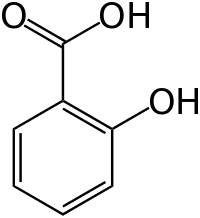
\includegraphics[width=.3\textwidth]{figuras/acido_salicilico.png}
\end{center}
\caption{Ácido salicílico}\label{fig:acid_salicilico}
\end{figure}

A acetilação ou etanoilação é o processo de introdução do grupo acetila (ou etanoila) em um composto
orgânico. O radical acetila possui o grupo metila (\ce{CH3}$-$) conectado por uma ligação simples a um
carbonila. O carbono do grupo carbonila possui um único elétron livre, com o qual forma uma ligação
com o radical R da molécula.

\begin{figure}[H]
\begin{center}
    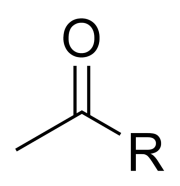
\includegraphics[width=.3\textwidth]{figuras/im1.png}
\end{center}
\caption{Grupo acetila ligado a uma cadeia carbônica.}\label{fig:im1}
\end{figure}

A seguir é explicada uma reação do ácido salicílico com utilização do anidrido acético como agente de
acetilação na produção de ácido acetilsalicílico. Essa síntese é a uma das mais reproduzidas, pois
possui características comerciais que são mais favoráveis às indústrias químicas devido a sua
eficiência e o seu baixo custo. Há a necessidade de um catalisador nessa reação e o descrito no
mecanismo a seguir é o ácido sulfúrico. Resumidamente, a reação entre um anidrido e um álcool (ou
hidroxiácido) gera um ácido carboxílico e um éster. Os ésteres são também derivados de ácido
carboxílico. Eles são majoritariamente apolares e insolúveis em água, entretanto são solúveis em
álcool. Eles se dispõem de pontos de fusão e de ebulição baixos por não apresentarem ligações de
hidrogênio. Sua produção advém da reação de um ácido carboxílico com um álcool, resultando em perda
de água.~\cite{SantosES}

\begin{figure}[H]
\begin{center}
    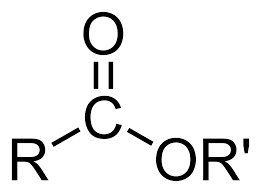
\includegraphics[width=.3\textwidth]{figuras/ester.png}
\end{center}
\caption{Forma generalizada de um éster}
\label{fig:ester}
\end{figure}

Dando início à síntese, o ácido sulfúrico irá agir na reação como um catalisador, sendo assim ele
irá se ionizar liberando um \ce{H+} que se ligará em um dos oxigênios presentes na molécula de
anidrido acético. Quando isso ocorre, o oxigênio que recebeu o hidrogênio deixa de fazer ligação
dupla com o carbono e consequentemente o carbono fica com três ligações, tornando-se um carbocátion.
Como o carbono está instável, ele busca a sua estabilidade na molécula de ácido salicílico com a
qual ele está reagindo. Portanto, o carbono liga-se na hidroxila do ácido salicílico, mas é
importante ressaltar que a hidroxila que ele irá se ligar é a hidroxila ligada diretamente ao anel
benzênico, devido as forças de atração. Na química orgânica, as ligações de acetilação tem
preferências para se ligarem em hidroxilas em posições orto e para, como é o caso do ácido
salicílico (posição orto da hidroxila). A formação da nova molécula de ácido salicílico com o
carbocátion do anidrido acético possui um oxigênio que contém três ligações, o qual se rearranja na
molécula se desprotonando para estabilizar, ou seja, o hidrogênio ligado a ele irá se ligar no
oxigênio que faz parte do anidrido acético, formando assim um ácido acético que irá se desprender da
molécula. A ligação de elétrons que estava ligada com a parte do ácido acético se direciona para o
respectivo carbono que estava fazendo tal ligação, mas antes disso o hidrogênio da hidroxila que
estava ligada a esse carbono volta para o catalisador (formando novamente o \ce{H2SO4}). Como o
carbono recebeu os pares de elétrons e o oxigênio da hidroxila perdeu o seu hidrogênio, acontece uma
dupla ligação entre o carbono e o oxigênio, dando origem a molécula de ácido acetilsalicílico.


% Remover '\newpage' caso a imagem a baixo altera sua posição
\newpage

\begin{figure}[H]
\begin{center}
    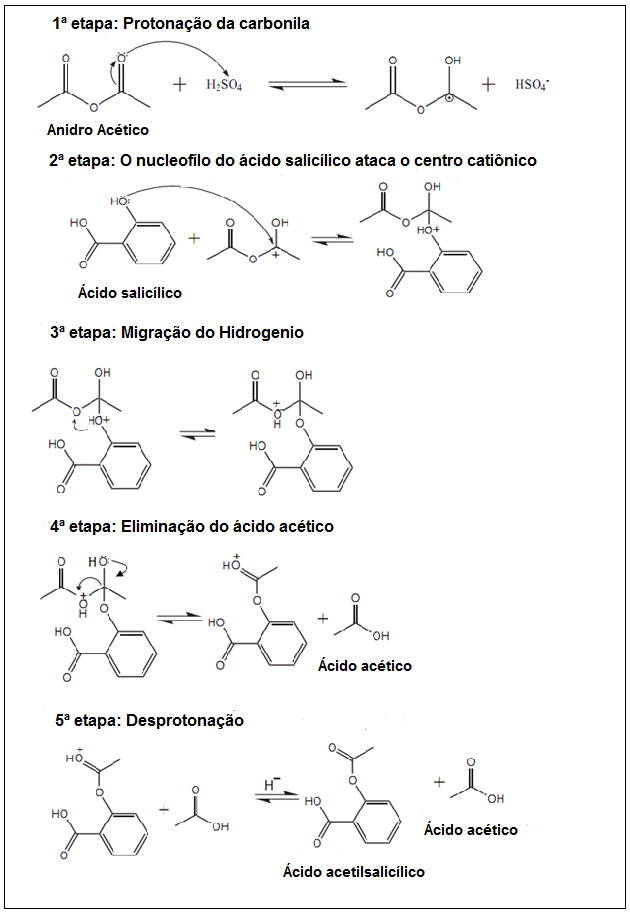
\includegraphics[width=1.1\textwidth]{figuras/im2_sintese.png}
\end{center}
\caption{Reação de síntese do ácido acetilsalicílico~\cite{Silva2010}}\label{fig:im2}%
\end{figure}

Segundo BRUICE (2006), a reação de carboxilação de Kolbe-Schmitt ficou conhecida como a primeira
etapa da síntese industrial de Aspirina$^\tiny{\textregistered}$. Ela consiste na reação do íon
fenolato com o dióxido de carbono, sob pressão, formando o ácido salicílico. Este por sua vez, ao
sofrer acetilação com o ácido acético forma o ácido acetilsalicílico.~\cite{Bruice2006}

Há diversas maneiras de sintetizar o ácido acetilsalicílico, sendo que a matéria prima para a
sintetização é o ácido salicílico e as variações ocorrem com os agentes de acetilação e os
catalisadores.

Em relação aos agentes de acetilação pode-se fazer uso também do cloreto de acetila e do ácido
acético glacial (com redução da água formada na reação) na síntese do ácido acetilsalicílico.  No
entanto, o procedimento envolvendo o ácido acético glacial requer longo tempo de aquecimento, apesar
de apresentar um custo inferior. Já o cloreto de acetila não é recomendado porque ele é muito
reativo. Ele se hidrolisa facilmente com a umidade do ar e em temperatura ambiente. O anidrido
acético é o agente de acetilação mais visionado nas reações de laboratório, porque sua velocidade de
hidrólise é suficientemente lenta para permitir que a acetilação seja realizada com maior
rendimento.~\cite{PERUCH2013}

Dentre a abundância de formas na produção de ácido acetilsalicílico a seguir estão apresentadas
algumas delas, em um esquema realizado pela  Associação Brasileria de Indústrias Químicas
(ABIQUIM), o qual envolveu a cadeia industrial da produção de Aspirina$^\tiny{\textregistered}$.

\begin{figure}[H]
\begin{center}
    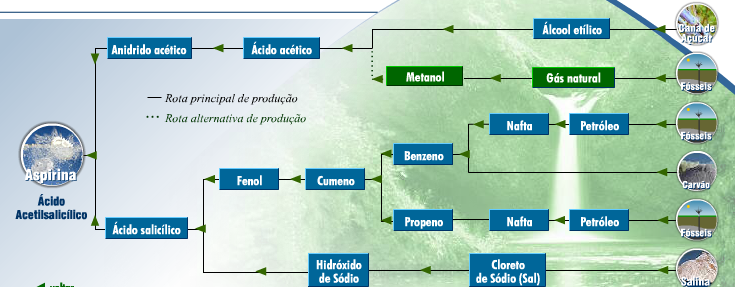
\includegraphics[width=1.10\textwidth]{figuras/abiquim.png}
\end{center}
\caption{Cadeia industrial da produção de Aspirina\R. (Fonte: ABIQUIM, 2009.~\cite{abiquim})}
\label{fig:abiquim}
\end{figure}

\subsection{Mecanismo de ação da Aspirina}

O ácido acetilsalicílico é um anti-inflamatório não esteroide (AINEs) ou não hormonal (AINHs), tendo
como propriedades analgésica, antipirética e anti-inflamatória. Além disso, possui um efeito
inibitório sobre as plaquetas no sangue e apresenta uma redução de 40\% no infarto do miocárdio
fatal e não fatal.~\cite{Palomo2008}

É usado para o alívio da dor e de quadros febris, tais como resfriados e gripes, para controle da
temperatura e alívio das dores musculares e das articulações. Também é usado nos distúrbios
inflamatórios agudos e crônicos, tais como artrite reumatoide, osteoartrite e espondilite
anquilosante.~\cite{bulaaspirina}

A atuação do ácido acetilsalicílico no organismo é de coibir a ação da ciclo-oxigenase. Essa ação
utiliza as enzimas COX-1 e COX-2, as quais transformam o ácido araquidônico em prostaglandinas, que
são responsáveis por induzir a dor e a febre. Esse ácido araquidônico é oriundo da ação enzimática
da Fosfolipase A2 sobre os fosfolipídios presentes nas membranas celulares. 

A plaqueta, importantíssima no processo de coagulação, é rica em COX-1 que, quando necessário,
produz prostaglandinas que são convertidas em Tramboxane A2 levando à formação de um coágulo. O
processo de coagulação se finda quando a Aspirina\R age na inflamação. Com o cessar da ação da
Aspirina\R no organismo, o processo de coagulação é retomado. Porém, uma vez que as plaquetas não
possuem núcleos elas não podem sintetizar uma nova COX para substituir a que foi inativa pela
Aspirina\R. Daí a ação anti-agregante plaquetária, que é um efeito irreversível. Entretanto, essa
ação irreversível não ocorre no endotélio vascular, pois este tem a capacidade de sintetizar as
novas moléculas. 

Devido a esse efeito inibitório da agregação plaquetária, o ácido acetilsalicílico pode aumentar a
tendência de sangramentos durante e após intervenções cirúrgicas (inclusive cirurgias de pequeno
porte, como por exemplo, extrações dentárias).~\cite{bulaaspirina}

Ademais, ao inibir a COX-2 ocorrerá o efeito anti-inflamatório, que diminuirá a inflamação vascular
no sítio da placa ateromatosa e esta, por sua vez, reduz a infiltração de células mononucleares na
placa de ateroma.~\cite{Grassi2012}

Algumas das funções das prostaglandinas estão na produção do muco estomacal, na coagulação sanguínea
e na manutenção da taxa de filtração glomerular nos rins. Como o fármaco (ácido acetilsalicílico)
inibe as enzimas COXs não há a produção das prostaglandinas, tendo como consequências alguns efeitos
no organismo.  Tais como, a úlcera péptica e uma posterior hemorragia digestiva, dependendo da
gravidade do quadro; a insuficiência renal aguda e problemas na coagulação. 

Após a medicação por via oral, o ácido acetilsalicílico é absorvido de forma rápida e completa no
trato gastrintestinal. Depois de absorvido e durante a sua absorção, o ácido acetilsalicílico é
convertido em ácido salicílico, que é o seu principal metabólito ativo. A quantidade máxima de
fármaco na corrente sanguínea do ácido acetilsalicílico é atingida após 10 a 20 minutos e a do ácido
salicílico após 0,3 a 2 horas. 

O ácido acetilsalicílico e o ácido salicílico possuem uma grande afinidade com as proteínas
plasmáticas, logo eles ligam-se extensivamente com tais proteínas e são distribuídos por todo o
organismo rapidamente.  O ácido salicílico passa para o leite materno e atravessa a placenta.

O ácido salicílico é eliminado principalmente por metabolismo hepático. Seus metabólitos incluem o
ácido salicilúrico, o glicuronídeo salicílico fenólico, o glicuronídeo salicilacílico, o ácido
gentísico e o ácido gentisúrico.

O metabolismo é restringido pela capacidade das enzimas hepáticas, sendo assim a cinética da
eliminação do ácido salicílico é dose-dependente. “A meia-vida de eliminação varia de 2 a 3 horas
após doses baixas até cerca de 15 horas com doses altas”~\cite{bulaaspirina}. O ácido salicílico e
seus metabólicos são excretados predominantemente por via renal. 

É importante frisar que esses anti-inflamatórios não esteroides (AINEs), do qual o ácido
acetilsalicílico faz parte, apenas inibem a produção de prostaglandinas na inflamação, mas eles não
cessam a mesma.

\subsection{Medicamentos de referência, genéricos e similares}\label{refgensim}

No mercado farmacêutico, medicamentos com o mesmo princípio ativo podem surgir com diferentes marcas
ou classificações. No caso do ácido acetilsalicílico, algumas são associadas a outras substâncias
como cafeína ou vitamina C. Outras possuem revestimentos de cápsula que buscam diminuir a agressão ao
sistema digestivo.~\cite{prade2006}

Com essas diferenças, os remédios são classificados como referência, genérico e similar. Os
medicamentos de referência, que também são conhecidos como “de marca”, são remédios que possuem
eficiência terapêutica, com qualidade e seguranças comprovadas cientificamente. São registrados
juntamente à Agência Nacional de substância Sanitária. Geralmente são medicamentos com novos
princípios ativos o que trazem novidades para o tratamento da doença.

Já os similares, além de possuir o mesmo princípio ativo do medicamento de referência, possui uma
identificação de nome comercial ou marca. A diferença é apresentada em alguns aspectos como
embalagem, rótulo, tamanho, validade e forma do produto. De acordo com a regulamentação da ANVISA,
dado uma prescrição médica os medicamentos de referência não podem ser substituídos por similares.

Para a possibilidade de troca desses medicamentos, ou seja, serem intercambiáveis, eles devem
apresentar um dos três testes: bioequivalência, biodisponibilidade e bioisenção. O estudo de
bioequivalência é sempre realizado entre o medicamento de referência e o estudado. Estas análises
tem o intuito de reafirmar a igualdade entre os produtos, proporcionando segurança e
eficiência.~\cite{ache2015}

\subsection{Titulação}\label{titulacao}

``Titulação é um procedimento no qual a quantidade de analito de uma amostra é determinada
adicionando-se uma quantidade conhecida de um reagente que reage completamente com o analito de uma
forma bem definida'' (HAGE, CARR. 2012)~\cite{Hage2012}.

Titulações volumétricas compreendem a medida de volume de uma solução padrão (de concentração
conhecida) necessária para reagir completamente com o analito.~\cite{Skoog2014}

Em uma titulação ácido-base, o titulado (analito) é um ácido e o titulante (solução ou composto com
os metros conhecidos) é uma base, ou vice-versa. Para saber quando e quanto de todo o analito
reagiu, é necessário adicionar um indicador ácido-base, uma substância química que muda de cor em
uma faixa conhecida de pH, ajudando a detectar o ponto estequiométrico ou ponto de equivalência.

``O ponto de equivalência é o ponto teórico alcançado quando a quantidade adicionada do titulante é
quimicamente equivalente à quantidade de analito na amostra''~\cite{Skoog2014}. O ponto final é o
ponto onde ocorre visualmente a percepção de alterações físicas (cor ou turbidez) pelo observador.

“Entre o ponto final da titulação e o ponto estequiométrico (teórico) sempre existirá uma pequena
diferença de volume do titulante chamada de Erro de Titulação”.~\cite{Ruy1999}

A reação de neutralização do AAS é dada abaixo:

\begin{center}
    \ce{C8O2H7COOH + NaOH -> C8O2H7COONa + H2O}
\end{center} 

Segundo Skoog et al. (2014), na titulação de um ácido fraco (HA) com uma base forte (\ce{NaOh} ou
\ce{KOH}) ocorrem as seguintes etapas:

\begin{enumerate}
    \item No início, a solução contém somente o analito, ácido fraco.
    \item Com a adição do titulante (até antes do ponto de equivalência), a solução contém uma série
        de tampões, entre a base conjugada formada da reação e o ácido fraco residual que permanece.
    \item No ponto de equivalência, a solução contém apenas o conjugado do ácido (um sal).
    \item Após o ponto de equivalência, o excesso de titulante básico reprime o caráter ácido ou
        alcalino do sal formado, produto da reação, sendo o pH resultante da concentração do excesso
        de titulante.
\end{enumerate}

\begin{figure}[H]
\begin{center}
    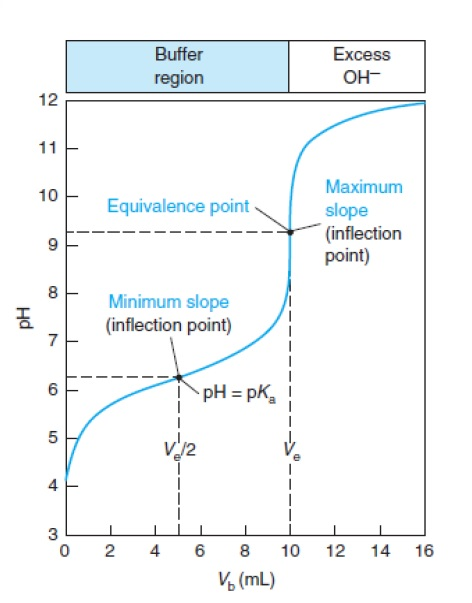
\includegraphics[scale=.9]{figuras/titulacao.jpg}
\end{center}
\caption{Curva de titulação Ácido fraco $\times$ Base forte}
\label{fig:curva_titulacao}
\end{figure}

\chapter{ELEMENTOS DO TEXTO}
\label{cap:elementos}

Este capítulo apresenta o uso básico de equações, figuras e tabelas no código da monografia, bem como o posicionamento das legendas, segundo as normas da UFLA.

\section{Utilizando Recursos do \LaTeX}

\subsection{Inserindo Comandos Definidos}

Esta subseção apresenta o uso de comandos definidos pelo usuário no preâmbulo do arquivo principal \LaTeX e alguns exemplos do modo matemático. Por exemplo, na texto a seguir é utilizado o comando  \verb+\defs+, definido anteriormente pelo próprio autor do texto:

\begin{quote}
Os conjuntos fundamentais da teoria são os \defs{conjuntos elementares}. Se $E$ é um conjunto elementar, $des(E)$ denota a descrição dessa classe de equivalência. Essa descrição é função do conjunto de atributos que define $R$. Note que, dados $x,y \in E$, onde $E$ é um conjunto elementar em $A$, $x$ e $y$ são indiscerníveis, i.e., no espaço $A=(U,R)$ não se consegue distinguir $x$ de $y$, pois $des(x) = des(y) = des(E)$. 
\end{quote}

\subsection{Inserindo Figuras}

A Figura~\ref{fig:exemplo} é apenas um exemplo de figura para que o usuário da classe possa saber como uma figura pode ser inserida e referenciada automaticamente no texto.É importante observar que legendas de figuras ficam abaixo de seu conteúdo.

\begin{figure}[!htb]
\centering
\caption{Uma Figura de Exemplo} %legenda

\includegraphics[scale=0.9]{gradpenguin}\\  % o 0.9 indica 90% do tamanho original
% pdfLaTeX aceita figuras no formato PNG, JPG ou PDF
% figuras vetoriais podem ser exportadas para eps e depois convertidas para pdf usando epstopdf
{\small Fonte: fonte da figura} %Fonte da imagem
\label{fig:exemplo} %rotulo para refencia
\end{figure}

\subsection{Inserindo Saídas de Comandos e Código}

A menos que sejam trechos pequenos, saídas de comandos, trechos de arquivos de configuração e código de aplicativos devem ser inseridos como figura, como mostrado, respectivamente, na Figura~\ref{fig:exemplocomando}, Figura~\ref{fig:exemploconfig} e Figura~\ref{fig:exemplocodigo1}. Para comandos e configuração, recomenda-se o uso do pacote {\tt fancyvrb}, o que pode ser visto na Figura~\ref{fig:exemplocomando} e Figura~\ref{fig:exemploconfig}.

Para inserção de código, recomenda-se o uso do pacote {\tt listings}, que permite melhor apresentação do mesmo, o que é mostrado na Figura~\ref{fig:exemplocodigo1}. Além disso, esses dois pacotes permitem a inserção de texto/código em arquivos externos, sem inclusão direta no arquivo \LaTeX. Isso pode ser verificado no exemplo de uso do {\tt listings} apresentado na Figura~\ref{fig:exemplocodigo2}

\begin{figure}[!htb]
\centering
\caption{Inserindo Comando} %legenda
\begin{Verbatim}[fontsize=\small]
$ dir monografia*
-rw-r--r--  1 joukim users   3650 Set 12 17:56 monografia.aux
-rw-r--r--  1 joukim users   6366 Set 12 17:43 monografia.bbl
-rw-r--r--  1 joukim users    290 Set 12 17:56 monografia.lof
-rw-r--r--  1 joukim users  27937 Set 12 17:56 monografia.log
-rw-r--r--  1 joukim users    194 Set 12 17:56 monografia.lot
-rw-r--r--  1 joukim users    715 Set 12 17:56 monografia.out
-rw-r--r--  1 joukim users 159243 Set 12 17:56 monografia.pdf
-rw-r--r--  1 joukim users   4559 Set 12 17:47 monografia.tex
-rw-r--r--  1 joukim users    964 Set 12 17:56 monografia.toc
\end{Verbatim} 
%$ - esse comentário é para não confundir editor de texto
{\small Fonte: fonte da figura} %Fonte da imagem
\label{fig:exemplocomando} %rotulo para refencia
\end{figure}

\begin{figure}[!htb]
\centering
\caption{Inserindo Trecho de Arquivo de Configuração} %legenda
\begin{Verbatim}[fontsize=\small]
// named.conf for Red Hat caching-nameserver
options {
        directory "/var/named";
        dump-file "/var/named/data/cache_dump.db";
        statistics-file "/var/named/data/named_stats.txt";
        // query-source address * port 53;
};
\end{Verbatim} 
{\small Fonte: fonte da figura} %Fonte da imagem
\label{fig:exemploconfig} %rotulo para refencia
\end{figure}


\begin{figure}[!htb]
\centering
\caption{Inserindo Código Diretamente no Arquivo \LaTeX} %legenda
\begin{lstlisting}
// exit the program
public void on_buttonExit_clicked() {
	System.exit(0);
}

// copy data
public void on_buttonCopy_clicked() {
	labelShow.setText(entryData.getText());
}

// print version of Java
public static void main(String[] args) {
	System.out.println(System.getProperty("java.fullversion"));
}
\end{lstlisting} 
{\small Fonte: fonte da figura} %Fonte da imagem
\label{fig:exemplocodigo1} %rotulo para refencia
\end{figure}


\begin{figure}[H]
\centering
\caption{Inserindo Código a Partir do Código-Fonte} %legenda
\label{fig:exemplocodigo2} %rotulo para refencia
\lstinputlisting{Hello.java}
{\small Fonte: fonte da figura} %Fonte da imagem
\end{figure}

\subsection{Inserindo Quadros e Tabelas}

Escrever um quadro ou tabela e referenciá-los é bem simples. Por exemplo o Quadro~\ref{tab:exemplo} ilustra a criação de um quadro, tendo aqui seu referenciamento no texto. É importante observar o posicionamento da legenda antes do corpo da tabela e da fonte após. Outros exemplos são mostrados na Tabela~\ref{tab:outro} e Tabela~\ref{tab:maisum}.

\begin{quadro}[htb]
  \begin{center}
    \caption{Exemplo de Quadro} 
    \label{tab:exemplo}
    \vspace{0.2cm}
    \footnotesize
    \begin{tabular}{|c|c|c|c|c|c|}
      \hline
      $U$ & $vitA$ & $vitC$ & $vitD$ & $prot$ & $lip$ \\
      \hline
      \hline
      $d_1$ & 1 & 3 & 4 & 2 & 3\\
      $d_2$ & 1 & 3 & 3 & 3 & 2\\
      $d_3$ & 1 & 3 & 4 & 3 & 1\\
      $d_4$ & 3 & 5 & 2 & 5 & 2\\
      $d_5$ & 4 & 5 & 2 & 5 & 1\\
      $d_6$ & 3 & 5 & 2 & 3 & 4\\
      $d_7$ & 4 & 4 & 1 & 3 & 2\\
      \hline 
    \end{tabular}
  \end{center}
  \centering {\small Fonte: fonte do quadro} %Fonte do quadro
\end{quadro}

\begin{table}[!htb]
\begin{center}
  \caption{Recursos do {\ttfamily syslog}}
  \label{tab:outro}
  \small
  \begin{tabular}{l|p{9cm}}
    \hline
    \rowcolor[gray]{.9}
    \bf Recurso & \bf {\em Daemons} Associados (Alguns Exemplos) \\
    \hline
    \hline
    \tt kern & \em kernel  \\
    \tt user & processos dos usuários ({\tt ntpd}) \\
    \tt mail & softwares relacionados com o correio eletrônico ({\tt sendmail})\\
    \tt daemon & {\em daemons} do sistema ({\tt gated}, {\tt inetd}, 
    {\tt named}, {\tt ntpd})\\
    \tt auth &  comandos relacionados à autorização e segurança 
    ({\tt login}, {\tt rlogin}, {\tt su}, {\tt passwd}) \\
    \tt lpr & spool de impressão ({\tt lpd})\\
    \tt news & sistema de notícias da usenet ({\tt nnrpd})\\
    \tt uucp & destinado ao {\tt uucp}\\
    \tt cron & relacionado ao {\em daemon} {\tt cron}\\
    \tt mark &  registros de data/hora gerados a intervalos regulares 
    ({\tt syslogd})\\
    \tt local0-7 & 8 tipos de mensagens locais \newline
    ({\tt tcpd -- local7}, {\tt sudo -- local2}, {\tt popper - local0}) \\
    \tt syslog &  mensagens internas ao {\tt syslog}\\
    \tt authpriv & mensagens privadas de autorização\\
    \tt ftp & associado ao {\tt ftpd} ({\em daemon} do {\tt ftp}) \\
    \tt * &  todos os recursos com exceção do {\tt mark}\\
    \hline
  \end{tabular}
\end{center}
\centering {\small Fonte: fonte da tabela} %Fonte da tabela
\end{table}

\begin{table}[!htb]
\caption{Opções do Comando {\ttfamily at}}
\label{tab:maisum}
\begin{center}
  \small
  \begin{tabular}{l|p{9cm}}
    \hline 
    \rowcolor[gray]{.9}
    \bf Opção & \bf Descrição\\
    \hline
    \hline 
    \tt -c & exibe os jobs registrados\\
    \tt -d & remove um job específico\\
    \tt -f & permite que os comandos sejam lidos a partir de um arquivo (não pela
    entrada-padrão)\\
    \tt -l & lista todos os jobs associados a um usuário\\
    \tt -m & envia um e-mail ao usuário quando o job for finalizado\\
    \hline \end{tabular}\\
\end{center}
\centering {\small Fonte: fonte da tabela} %Fonte da tabela
\end{table}

\subsection{Inserindo Equações}

Equações devem ser numeradas, com a numeração, em parênteses à direita da mesma. Isso é ilustrado na Equação~\ref{eq:exemplo}.

\begin{equation}
\label{eq:exemplo}
f'(x) = \int^{x^2}_{x^{-1}} xdx 
\end{equation}


\section{Usando Referências}
A equipe do curso não impõe normas rígidas para o formato a ser adotado nas referências bibliográficas, desde que seja usado um padrão acadêmico conhecido. Caso os autores não possuam um padrão preferencial, recomenda-se o formato estipulado pela ABNT \cite{NBR6023:2002}. A Biblioteca Central da UFLA disponibiliza um manual \cite{BIBUFLA2001} que orienta o uso dessas normas. Se os autores estiverem utilizando \LaTeX, recomenda-se o uso do pacote Abn\TeX\footnote{Disponível em \url{http://abntex.codigolivre.org.br/}.} \cite{Weber2003}. 

Obviamente, recomenda-se a leitura de textos sobre a escrita acadêmica e produção de trabalhos de conclusão para garantir não só qualidade estética e de formatação, mas também de conteúdo. Entre outros, pode-se recomendar a leitura de \cite{Silva2005}, \cite{Martins2000}, \cite{Gil2002}, \cite{Franca2001}, \cite{Eco1996}, \cite{Moura1998}, \cite{Booth2000}, \cite{Hexsel2004}, \cite{Porto2002} e \cite{Henz2003}. 


\chapter{Conclusão}

A quantidade de ácido acetilsalicílico foi determinada nos seguintes comprimidos: Aspirina\R, 
Melhoral\R, genérico e AAS Infantil.

Foram realizados dois experimentos. Para o primeiro experimento, todas as massas calculadas
encontraram-se fora do intervalo aceitável de $\pm$ 5\%, segundo a Farmacopeia Brasileira, o qual
foi adotado neste experimento. O resultado mais próximo do real foi o do genérico, com um erro
relativo de de $7,148\%$ e houve uma maior descrepância nos dados da Aspirina\R, com erro relativo
de $20,104\%$.

No segundo experimento, todos os resultados encontram-se dentro do intervalo aceitável, exceto o
genérico, o qual aprensentou erro relativo de $6,643\%$. Já o AAS Infantil foi o que apresentou mais
proximidade em relação ao real, tendo um erro relkativo de $3,537\%$.


%==============================================================================
% Incluindo bibliografia
%\bibliographystyle{plain}             % estilo para labels em numeros
%\bibliographystyle{alpha}             % estilo para labels em iniciais
\bibliographystyle{abntex2-alf}           % estilo para referências usando ABNT, 
                                       % precisa instalar o abntex para usar!!!

%inclui Referências Bibliográficas
%inclui Referências Bibliográficas
\referencias
\bibliography{refbib}			% arquivo exemplo refbib.bib
%==============================================================================
% Incluindo anexos num1erados com letras maiusculas.
%\apendices
\apendice{O que são apêndices}
\label{cap:apendice}

Um apêndice é um suporte elucidativo e ilustrativo do texto principal. Sua função é agrupar elementos que são úteis à compreensão do texto e que, no entanto, podem ser apresentados à parte sem prejuízo à compreensão. É útil para a apresentação de modelagens, diagramas extensos, listagens de código-fonte de programas e demais elementos que o autor julgar necessário à complementação do tema abordado no texto principal.


%==============================================================================
% Fim do texto
\end{document}
